
\subsection{Carbon Number of \ce{O_x} Producing Degradation Products} \label{ss:c_number} %comparison by carbon number breakdown

\begin{figure}
    \begin{center}
        \includegraphics[width=\textwidth]{img/carbon_percent_total_Ox_production}
    \end{center}
    \caption{Pentane and toluene daily \ce{O_x} production percentage contributions by carbon number of degradation products.}
    \label{f:percent_carbon}
\end{figure}

\begin{figure}
    \begin{center}
        \includegraphics[width=\textwidth]{img/TOL_MCM_CRI_HO2x_intermediates}
        \caption{The \ce{HO2_x} production budgets from toluene degradation attributed to the responsible reactions in (a) MCM v3.2 and (b) CRI v2.}
        \label{f:toluene_HO2x}
    \end{center}
\end{figure} 

The different NMVOC \ce{O_x} production time profiles in Figure \ref{f:TOPP_dailies} results from the different rates at which the NMVOCs break up into smaller fragments \citep{Butler:2011}.
The percent contributions from the degradation products amount of carbon on daily \ce{O_x} production during pentane and toluene degradation is illustrated in Figure \ref{f:percent_carbon}.

Figure \ref{f:percent_carbon} indicates that near-explicit mechanisms retain a larger influence on \ce{O_x} production of degradation products having the same number of carbons as the emitted NMVOC throughout the model run than less-explicit mechanisms.
Toluene degradation in MOZART-4 is an exception.
Despite the large influence of C7 degradation products the daily \ce{O_x} production from toluene in MOZART-4 is practically zero after the fourth day.
\todo{add sentence about reactive carbon loss results -> this must be due to a quick breakdown but need to prove this.}

The impact of C1 and C2 degradation products increases over the run.
Emitted NMVOCs are oxidised to these smaller fragments quicker in the less-explicit mechanisms implying less carbon to fuel \ce{O_x} production.
\todo{slower in explicit mechanisms? Reactive carbon analysis needed for this claim}

C1 and C2 degradation products are the sole influence on \ce{O_x} production from alkane degradation in CBM-IV and CB05.
Alkane degradation is depicted using PAR, whose degradation consists of mechanism species having either one or two carbon atoms.
PAR represents singly bonded carbons and alkane emissions are scaled by the carbon number to account for increased \ce{O_x} production with alkane carbon number.
\citet{Hogo:1989} and \citet{Yarwood:2005} contain details for the CBM-IV and CB05, whilst Section \ref{ss:mechanisms} has a brief summary.

CRI v2 and RACM2 toluene degradation differs from toluene degradation in all other mechanisms as maximum \ce{O_x} production is reached on the second day. 
In RACM2 this is due to the degradation into smaller products happening at a slower pace than in other mechanisms.
\todo{confirm this with reactive carbon analysis}

Toluene C2 degradation products in CRI v2 have a larger impact than in the MCM.  
Figure \ref{f:toluene_HO2x} illustrates the \ce{HO2_x} production budget allocated to the responsible reactions in MCM v3.2 and CRI v2. 
The \ce{HO2_x} family consists of \ce{HO2} and \ce{HO2NO2}.
\ce{HO2_x} production influences \ce{O_x} production through \ce{HO2} converting NO to \ce{NO2} via \reactionref{r:HO2_NO}.
\mbox{Figure \ref{f:toluene_HO2x}} shows more \ce{HO2_x} production from the reaction of CARB3 and OH in CRI v2 than its corresponding MCM v3.2 reaction (\mbox{GLYOX + OH}).

Glyoxal is represented as CARB3 in CRI v2 and GLYOX in MCM v3.2, but there are many differences in the chemistry of these species.
In CRI v2, CARB3 is only produced from aromatic degradation whilst GLYOX is also a degradation product of other non-aromatic NMVOCs in MCM v3.2. 

CRI v2 glyoxal degradation is through reaction with OH radical and photolysis whilst extra degradation options are available in MCM v3.2. 
Moreover, the rate constant for the reaction with OH radical in CRI v2 is $\sim$ $15$\% faster than in MCM v3.2. 

Glyoxal has three available photolysis pathways in MCM v3.2 and only one in \mbox{CRI v2}. 
These photolysis pathways and their rate parameters are outlined in Table \ref{t:glyoxal}. 
The additional photolysis pathways in MCM v3.2 are non-\ce{HO2_x} producing pathways leading to less \ce{HO2_x} production.

{
    \renewcommand{\arraystretch}{1.3}
    \begin{table}
        \begin{center}\small
            \begin{tabular}{lP{6.8cm}P{3.0cm}}
                \hline \hline
                \textbf{Mechanism} & \textbf{Photolysis Pathway} & \textbf{Rate Parameter} \\ \hline \hline
                \multirow{3}{*}{MCM v3.2} & GLYOX + hv = CO + CO + H2 & J$_{31}$ \\
                & GLYOX + hv = HCHO + CO & J$_{32}$ \\
                & GLYOX + hv = CO + CO + HO2 + HO2 & J$_{33}$ \\ \hline
                CRI v2 & CARB3 + hv = CO + CO + HO2 + HO2 & J$_{33}$ \\ \hline \hline
            \end{tabular}
            \caption{Glyoxal photolysis in MCM v3.2 and CRI v2 with specified rate parameters.}
            \label{t:glyoxal}
        \end{center}
    \end{table}
}

The combination of the higher rate constant for the glyoxal reaction with OH radical and additional \ce{HO2_x} production during photolysis are responsible for the higher \ce{HO2_x} production in CRI v2. 

\subsection{Radical Production and Consumption Budgets} \label{ss:radicals}

\ce{O_x} production is directly to the conversion of NO to \ce{NO2} by peroxy radicals. 
Moreover, in this study maximum \ce{O3} production was achieved by emitting the amount of NO required to balance the radical source at each time step. 
A radical family for each mechanism was used to investigate the processes affecting production and loss budgets. 
This radical family includes all radical species and species involved in quick production and consumption cycles, such as PAN species and \ce{HO2NO2}.

\begin{figure}
    \begin{center}
        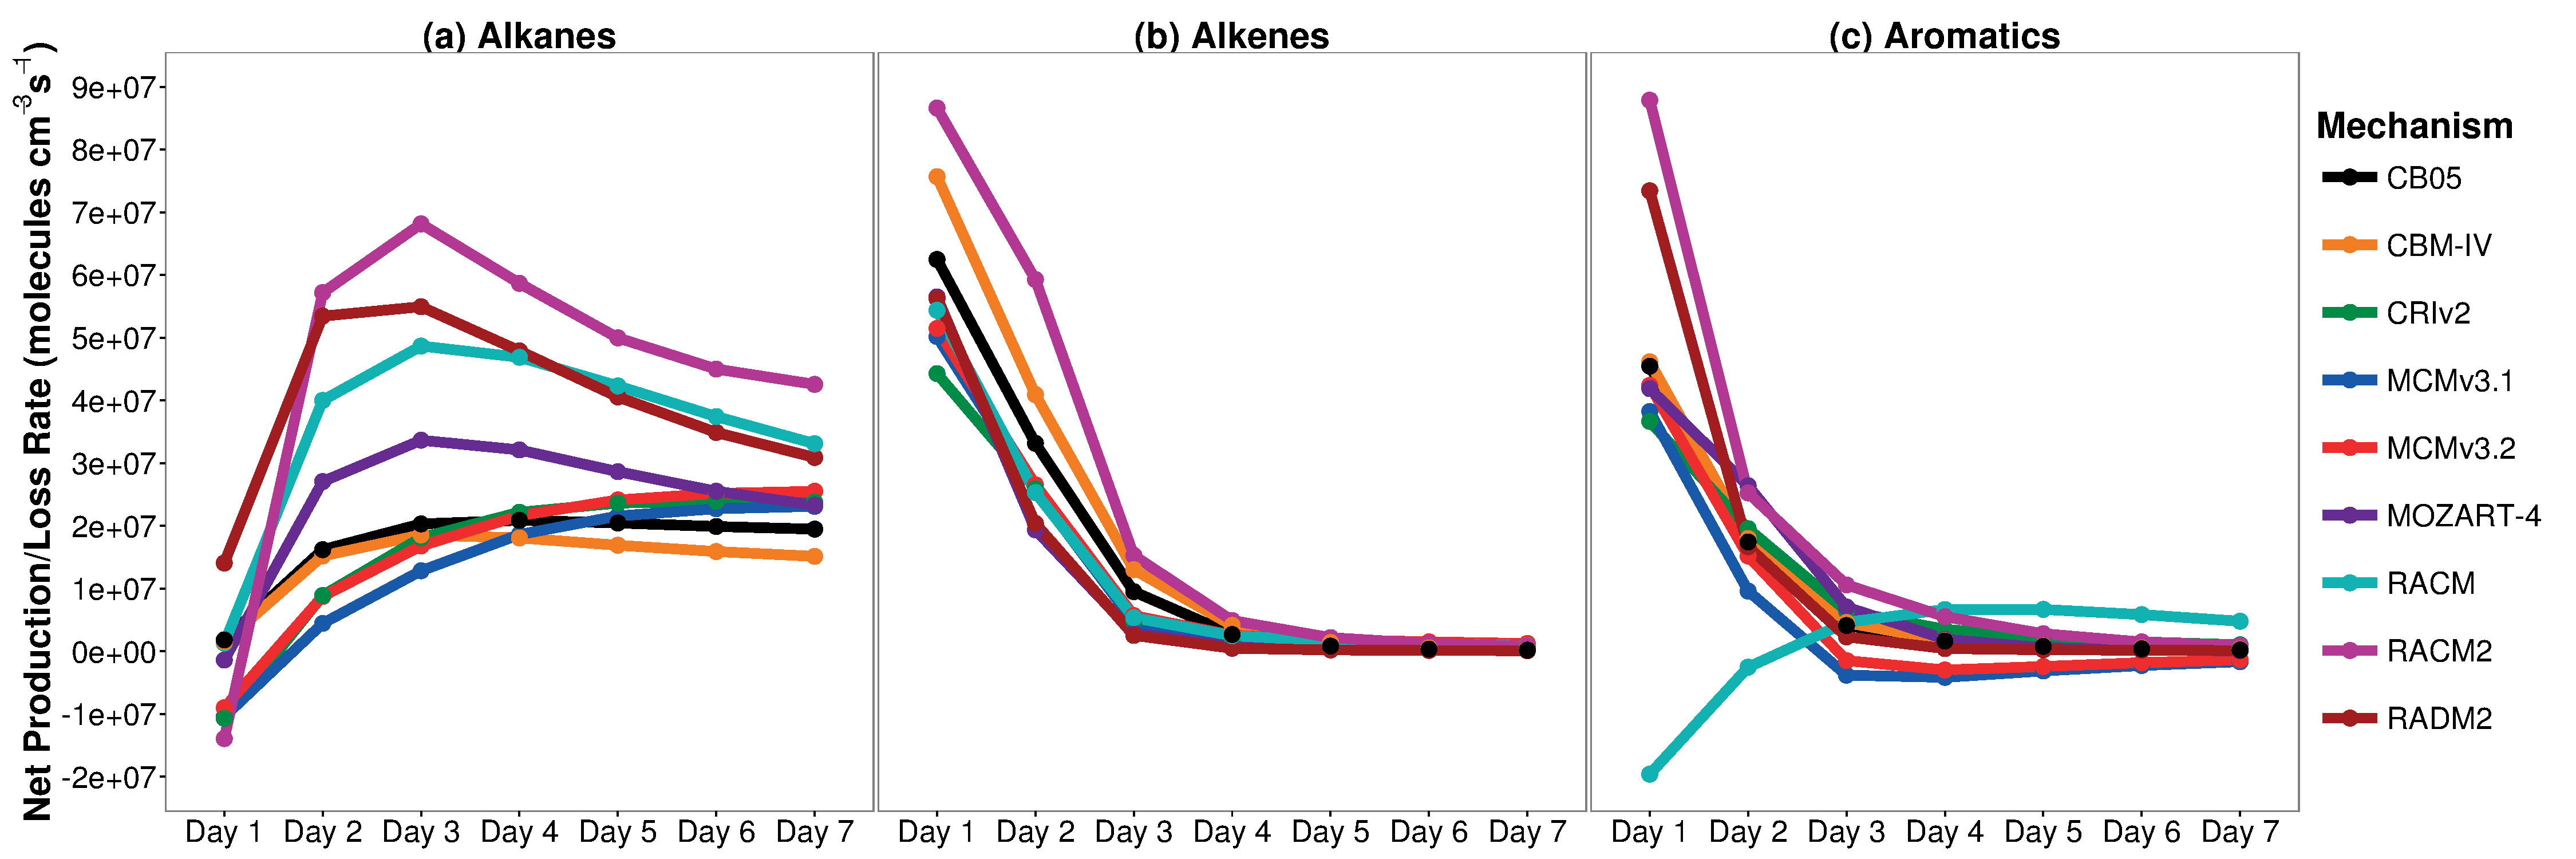
\includegraphics[width=\textwidth]{img/Net_radical_budgets}
    \end{center}
    \caption{The day-time net budget contribution of (a) alkane, (b) alkene and (c) aromatic degradation on the radical family in each mechanism.}
    \label{f:net_radical_budgets} 
\end{figure} 

\begin{figure}
    \begin{center}
        \includegraphics[width=\textwidth]{img/pentane_radical_budgets}
    \end{center}
    \caption{The processes influencing the radical family production and consumption budgets during pentane degradation are illustrated for (a) MCM v3.2, (b) MCM v3.1, (c) CRI v2, (d) RADM2, (e) RACM, (f) RACM2, (g) MOZART-4, (h) CBM-IV and (i) CB05.}
    \label{f:pentane_radical_budgets}
\end{figure}

\begin{figure}
    \begin{center}
        \includegraphics[width=\textwidth]{img/toluene_radical_budgets}
    \end{center}
    \caption{The processes influencing the radical family production and consumption budgets during toluene degradation is illustrated for (a) MCM v3.2, (b) MCM v3.1, (c) CRI v2, (d) RADM2, (e) RACM, (f) RACM2, (g) MOZART-4, (h) CBM-IV and (i) CB05.}
    \label{f:toluene_radical_budgets} 
\end{figure} 

The day-time net radical production and loss budgets due to alkane, alkene and aromatic degradation is shown in Figure \ref{f:net_radical_budgets}. 
The largest differences arise from alkane and aromatic degradation. 
Pentane and toluene radical budgets are attributed to the responsible processes in Figures \ref{f:pentane_radical_budgets} and \ref{f:toluene_radical_budgets} to determine the source of these differences.

In general, photolysis is the major radical production process and the reactions of radicals with other species, such as NO and \ce{HO2}, is the main radical sink. 
Reduced mechanisms include other processes to maintain radical production.

Figure \ref{f:pentane_radical_budgets} shows that initial VOC oxidation contributes to radical production in RADM2. 
This is represented by
\begin{reactionlist}
    \reactionitem{HC5 + OH}{HC5P + 0.25 XO2 + H2O}{new}{r:HC5_OH}
\end{reactionlist}
where HC5P is the pentyl peroxy radical and XO2 is an operator species which accounts for extra NO to \ce{NO2} conversions. 
XO2 is included in the radical family as it functions as a peroxy radical. 
This additional radical production pathway is responsible for the net first day radical production in RADM2.

The reactions of radicals lead to large net radical production in RACM after the first day. 
The main source being the reaction of HC5P with NO, 
\begin{center}
\refstepcounter{reaction}\label{r:HC5P_NO}
    \begin{tabular}{l@{\hskip 0.3cm}c@{\hskip 0.3cm}l@{\hskip 0.2cm}r}
        HC5P + NO & \reaction & 0.021 HCHO + 0.211 ALD + 0.722 KET & \reactionref{r:HC5P_NO} \\
        & & \hspace{2mm} + 0.599 HO2 + 0.031 MO2 + 0.245 ETHP & \\
        & & \hspace{2mm} + 0.334 XO2 + 0.124 ONIT + 0.876 NO2 &
    \end{tabular}
\end{center}
where HO2, MO2, ETHP and XO2 are the produced radical species. 
The larger net RADM2 and RACM radical production in Figure \ref{f:net_radical_budgets} is traced back to the extra radical production from reactions \reactionref{r:HC5_OH} and \reactionref{r:HC5P_NO} respectively.

Radical production in CBM-IV and CB05 is largely impacted by NMVOC initial oxidation and production from other radical reactions. 
Pentane degradation in these mechanisms is very similar and the CB05 reactions are considered here. 

Initial pentane degradation is via the PAR reaction with OH,
\begin{center}
\refstepcounter{reaction}\label{r:PAR_OH}
    \begin{tabular}{l@{\hskip 0.3cm}c@{\hskip 0.3cm}l@{\hskip 0.2cm}r}
        PAR + OH & \reaction & 0.87 XO2 + 0.13 XO2N + 0.11 HO2 + 0.06 ALD2 & \reactionref{r:PAR_OH} \\
        & & \hspace{2mm}  + 0.76 ROR + 0.05 ALDX - 0.11 PAR &
    \end{tabular}
\end{center}
where XO2, HO2 and ROR are the produced radical species. 
The mechanism species ROR decomposes immediately to either HO2 or \mbox{0.96 XO2 + 0.04 XO2N + 0.94 HO2 + 0.6 ALD2 + 0.02 ROR + 0.5 ALDX - 2.1 PAR}, once again XO2, HO2 and ROR are the produced radical species. 
The very fast decomposition of ROR and the use of XO2 to rapidly convert NO to \ce{NO2} leads to a rapid loss of radicals. 
The large production and consumption processes are balanced so that the net radical production correlates with that of the MCM v3.2.

The first day net radical production due to aromatic degradation are overestimated using RADM2 and RACM2 chemistry and underestimated in RACM. 
The RACM underestimation results from the degradation chemistry discussed in Section \ref{sss:RACM_aromatic}.

Figure \ref{f:toluene_radical_budgets} indicates that the RACM2 overestimation is due to radical production from reactions that do not involve radicals. 
The ozonolysis of the unsaturated dicarbonyl mechanism species DCB1 and DCB2 as well as the epoxy mechanism species EPX are additional reactions used to produce radicals.

The MCM v3.2 species TLEPOXMUC is analogous to EPX in RACM2. 
The ozonolysis rate constants are \mbox{$5 \times 10^{-18}$} and \mbox{$1 \times 10^{-16}$ cm$^3$ s$^{-1}$} respectively. 
The RACM2 rate constant is 20 times larger than that of the MCM v3.2 leading to excess radical production in RACM.

The ozonolysis of dicarbonyl species are included in RACM2 based on the recommendations of \citet{Bierbach:1994}. 
Dicarbonyl ozonolysis was not included in the MCM due to the uncertainties of these reactions \citep{Bloss:2005}.  
This additional radical source leads to larger net radical production.

